
\section*{Slides additionnels}

\begin{frame}{Structure de séquences}{Spécification}
  \begin{definition}[Spécification séquentielle d'une séquence]
  Soit une série d'opérations $H$ produisant la séquence
  $s(H) = \{p_1,\, p_2 \ldots p_k\}$ avec $p_{1..k} \in \mathcal{P}$ où
  $\mathcal{P}$ est un ensemble muni d'un ordre
  dense $(\mathcal{P},\,<_\mathcal{P})$ tel que : \\
  $\forall p\in\mathcal{P},\, p_\vdash <_\mathcal{P} p <_\mathcal{P} p_\dashv $
  \hfill et \ \
  $p_\vdash <_\mathcal{P} p_1 <_\mathcal{P} p_2 <_\mathcal{P} \ldots
  <_\mathcal{P} p_k <_\mathcal{P} p_\dashv$.
  
  \vspace{0.25cm}

  \noindent L'insertion d'un élément $e$ en position $i$ dans la séquence $s(H)$
  est définie de la façon suivante :
  \begin{equation}
    \small
    s(H \cup INSERT(i,\, e)) \rightarrow s(H) \cup 
    \begin{cases}
      \{p,\, p_\vdash <_\mathcal{P} p <_\mathcal{P} p_\dashv \} & i = 0 \wedge |s(H)| = 0\\
      \{p,\, p_\vdash <_\mathcal{P} p <_\mathcal{P} p_1 \} & i = 0 \wedge |s(H)|>0\\
      \{p,\, p_k <_\mathcal{P} p <_\mathcal{P} p_\dashv \} & i = k\\
      \{p,\, p_i <_\mathcal{P} p <_\mathcal{P} p_{i+1} \} & sinon
    \end{cases}
  \end{equation}

  \noindent La suppression de l'élément en position $i$ dans la séquence $s(H)$
  est définie de la façon suivante :
  \begin{equation}
    \small
    s(H \cup DELETE(i)) \rightarrow s(H) \setminus \{ p_i \}
  \end{equation}
\end{definition}
\end{frame}


\begin{frame}{Structure de séquences}{Complexité temporelle des accès}
  
  \begin{center}
    
\small
\begin{tabularx}{0.7\textwidth}{@{}Xc@{}}
  \toprule
  \textsc{Comportement d'édition} & \textsc{Temps} \\
  & \ \ \ \ \ \ \ \ \ \textsc{lookup} \ \ \ \ \ \ \ \ \ \\ \midrule
  Édition aléatoire & $\mathcal{O}(2^{\sqrt{\log I}})$ \\
  Édition monotone / pire cas & $\mathcal{O}(I)$ \\ \bottomrule
%%  Worst case & $\mathcal{O}(I)$ \\ \bottomrule
\end{tabularx}


  \end{center}
  
  Fonction qui permet de passer d'une structure de séquence à une structure
  d'arbre, et inversement.
  
  \vspace{0.25cm}%
  \begin{center}%
  \begin{tikzpicture}[scale=0.9]
  \newcommand\X{30pt}
  \newcommand\Y{45pt}

  \small
  \draw[dashed, thick] (0pt,0pt) -- node[anchor=south east]{0} (-3.5*\X,-1*\Y);
  \draw[thick, color=darkblue] (0pt,0pt) --
  node[anchor=west]{\DARKBLUE{1}} (-2.5*\X,-1*\Y);
  \draw[thick] (-2.5*\X,-1*\Y) -- node[anchor=east]{3} (-1.5*\X,-2*\Y);
  \draw[thick] (-2.5*\X,-1*\Y) -- node[anchor=east]{7} (-0.5*\X, -2*\Y);
  \draw[thick] (-2.5*\X,-1*\Y) -- node[anchor=west]{11} (0.5*\X,-2*\Y);
  \draw[thick, color=darkblue](0pt,0pt) -- 
  node[anchor=west]{\DARKBLUE{5}} ( 1.5*\X,-1*\Y);
  \draw[thick, color=darkblue] (1.5*\X,-1*\Y) -- 
  node[anchor=west]{\DARKBLUE{4}} (2.5*\X,-2*\Y);
  \draw[dashed, thick] (0pt,0pt) -- node[anchor=south west]{8} ( 3.5*\X,-1*\Y);

  \draw[->, color=darkblue] (-2.5*\X,-1*\Y) -- (-2.5*\X,-10-1*\Y);
  \draw[->] (-1.5*\X,-2*\Y) -- (-1.5*\X,-10-2*\Y);
  \draw[->] (-0.5*\X,-2*\Y) -- (-0.5*\X,-10-2*\Y);
  \draw[->] ( 0.5*\X,-2*\Y) -- ( 0.5*\X,-10-2*\Y);
  \draw[->, color=darkblue] ( 1.5*\X,-1*\Y) -- ( 1.5*\X,-10-1*\Y);
  \draw[->, color=darkblue] ( 2.5*\X,-2*\Y) -- ( 2.5*\X,-10-2*\Y);

  \draw[fill=white, draw=darkblue](-2.5*\X,-14-1*\Y)
  node{\DARKBLUE{\textbf{Q}}}+(-4pt,-4pt)rectangle+(4pt,4pt);
  \draw[fill=white](-1.5*\X,-14-2*\Y)node{\textbf{W}}+(-4pt,-4pt)rectangle+(4pt,4pt);
  \draw[fill=white](-0.5*\X,-14-2*\Y)node{\textbf{E}}+(-4pt,-4pt)rectangle+(4pt,4pt);
  \draw[fill=white]( 0.5*\X,-14-2*\Y)node{\textbf{R}}+(-4pt,-4pt)rectangle+(4pt,4pt);
  \draw[fill=white, draw=darkblue]( 1.5*\X,-14-1*\Y)
  node{\DARKBLUE{\textbf{T}}}+(-4pt,-4pt)rectangle+(4pt,4pt);
  \draw[fill=white, draw=darkblue]( 2.5*\X,-14-2*\Y)
  node{\DARKBLUE{\textbf{Y}}}+(-4pt,-4pt)rectangle+(4pt,4pt);

  \draw[fill=darkblue] (  0pt,  0pt) circle (1pt);
  \draw[fill=black] (-3.5*\X,-1*\Y) circle (1pt);
  \draw[fill=white, draw=darkblue] (-2.5*\X,-1*\Y) circle (1pt);
  \draw[fill=white] (-1.5*\X,-2*\Y) circle (1pt);
  \draw[fill=white] (-0.5*\X,-2*\Y) circle (1pt);
  \draw[fill=white] ( 0.5*\X,-2*\Y) circle (1pt);
  \draw[fill=white, draw=darkblue] ( 1.5*\X,-1*\Y) circle (1pt);
  \draw[fill=white, draw=darkblue] ( 2.5*\X,-2*\Y) circle (1pt);
  \draw[fill=black] ( 3.5*\X,-1*\Y) circle (1pt);

  \draw[->, very thick, densely dashdotted] (15-2.5*\X,-1*\Y) --
  node[anchor=south]{\textbf{explore}} (-20+1.5*\X, -1*\Y) -- (-20+2.5*\X, -2*\Y);


\end{tikzpicture}
  \end{center}%
  \vspace{0.25cm}

  \begin{itemize}
  \item Linéaire dans le cas monotone qui est aussi le pire cas.
  \item [$\rightarrow$] Heureusement, ce coût peut souvent être réduit.
  \end{itemize}
  
\end{frame}


\begin{frame}{Structure de séquences}{Effets de la concurrence}
  \vspace{-0.5cm}
  \begin{center}
    \includegraphics[angle=-90, width=\textwidth]{img/replication/latency.eps}
  \end{center}
\end{frame}


%% WORST CASE SLIDE LSEQ

